\documentclass[12pt]{report}

\setlength{\textwidth}{6.5in}
\setlength{\textheight}{8.5in}
\setlength{\evensidemargin}{0in}
\setlength{\oddsidemargin}{0in}
\setlength{\topmargin}{0in}

\setlength{\parindent}{0pt}
\setlength{\parskip}{0.1in}

% packages
\usepackage{bookmark}
\usepackage{acro}
\usepackage{graphicx}
\usepackage{listings}
\graphicspath{ {images/} }
\usepackage{upgreek}
\usepackage{caption}
\usepackage[nameinlink]{cleveref}
\usepackage{setspace}
%\usepackage{subcaption}
\usepackage{subfig}
\captionsetup[figure]{font=scriptsize, labelfont=bf}

%Redefining chapter heads
\makeatletter
\def\@makechapterhead#1{%
  %%%%\vspace*{50\p@}% %%% removed!
  {\parindent \z@ \raggedright \normalfont
    \ifnum \c@secnumdepth >\m@ne
        \huge\bfseries \@chapapp\space \thechapter
        \par\nobreak
        \vskip 20\p@
    \fi
    \interlinepenalty\@M
    \Huge \bfseries #1\par\nobreak
    \vskip 40\p@
  }}
\def\@makeschapterhead#1{%
  %%%%%\vspace*{50\p@}% %%% removed!
  {\parindent \z@ \raggedright
    \normalfont
    \interlinepenalty\@M
    \Huge \bfseries  #1\par\nobreak
    \vskip 40\p@
  }}
\makeatother
% end redefinition

% listings stuff
\renewcommand{\lstlistingname}{Algorithm}
\renewcommand{\lstlistlistingname}{List of \lstlistingname s}
\crefname{listing}{algorithm}{algorithms}
\Crefname{listing}{Algorithm}{Algorithms}
\lstset{
  numbers=left,
  stepnumber=5,    
  firstnumber=1,
  numberfirstline=true
}
% end listings stuff

% Acronyms
%\DeclareAcronym{io}{
%	short = I/O,
%	long = Input/Output,
%	class = acron
%}

\newcommand{\textsub}{\textsubscript}
\newcommand{\textsup}{\textsuperscript}
\def \doctitle {Simulation of Multi-input gates with Distinguishing X’s and X-Trees}

\begin{document}

\thispagestyle{empty}
\pagenumbering{roman}
\begin{center}

% TITLE
\pdfbookmark{Title Page}{}
{\Large 
\doctitle
}

\vfill

Ryan D. Burrow

\vfill

ECE 5505 Final Report

\vfill

\date{\today}

\vfill

Keywords: Testing and Verification, Logic Simulation, Distinguishing X's\\

\end{center}

\pagebreak

% Navigation information

\pdfbookmark{Table of Contents}{toc}
\tableofcontents
\pagebreak

\pdfbookmark{List of Figures}{lof}
\listoffigures

%\pdfbookmark{List of Tables}{lot}
%\listoftables
%
%\pdfbookmark{List of Algorithms}{loc}
%\lstlistoflistings
%\pagebreak

\pdfbookmark{List of Acronyms}{loa}
\printacronyms[include-classes=acron,name=List of Acronyms]
\pagebreak

\pagenumbering{arabic}
\pagestyle{myheadings}

% Content
\doublespacing

%reset acronyms, define them here
\acresetall

\chapter{Introduction} \label{introduction}

\section{Overview}

The goal of this project was to transform the previous project, which implemented a simulator of circuits containing distinguishing X’s, but only on dual input gates, for gates containing more than 2 inputs; the process of implementing this and the challenges of doing so will be discussed in \cref{sec:mig}. Another goal of this project was to implement some features that would help gain information from X values that were not squashed and were propagated to the output. The mechanism that was chosen to do this was named an X-Tree, and is a list of all the distinguishing X’s that make up an X value at any gate in the circuit. In addition, the first occurrence of each distinguishing X value and its inverse is tracked in two separate lists, to help identify key gates in the propagation path; this is covered in \cref{sec:xtree}. The final step to help obtain more information about these values was to implement an interface that would allow a user to interact with the circuit and inspect specific gates, as well as manipulate their output to see the effect on the circuit; this will be discussed more in \cref{sec:ui}.

\section{Background Research}

\cite{efficient-error}
\cite{multiple-defect}
\cite{incremental}
\cite{exclusive-test}
\cite{modeling-unknown}

\chapter{Multi-input gates}
\label{sec:mig}

\section{Overview}

\section{AND/OR}

\cref{fig:and-ul}
\cref{fig:xtree-ckt}

\begin{figure}[h]	
	\subfloat[]{\label{fig:and-ul}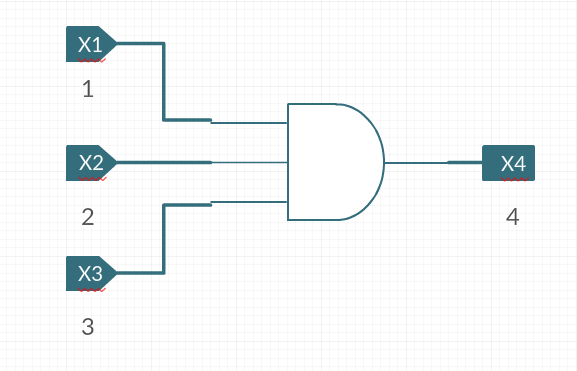
\includegraphics[width=0.5\textwidth]{3-input-and-ul.png}}
	\subfloat[]{\label{fig:and-ur}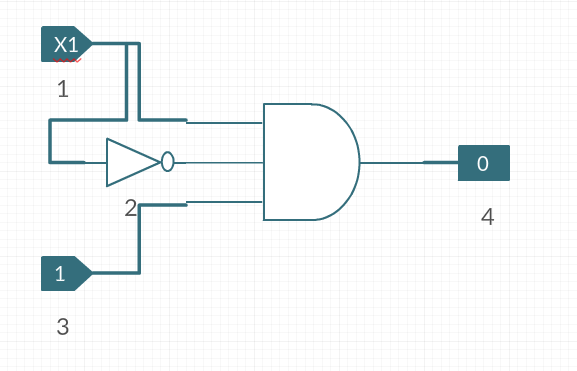
\includegraphics[width=0.5\textwidth]{3-input-and-ur.png}}
	\newline
	\subfloat[]{\label{fig:and-ll}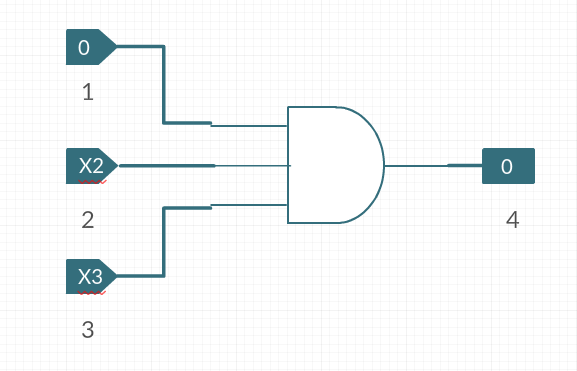
\includegraphics[width=0.5\textwidth]{3-input-and-ll.png}}
	\subfloat[]{\label{fig:and-lr}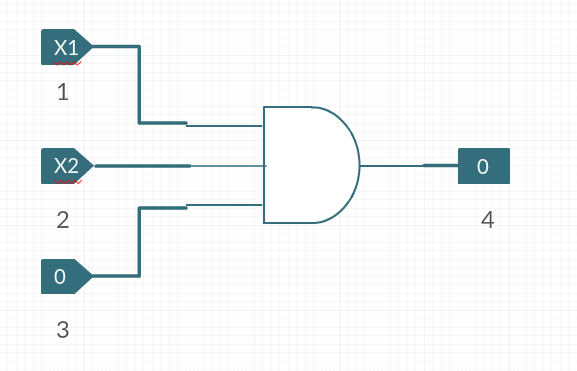
\includegraphics[width=0.5\textwidth]{3-input-and-lr.png}}
	\label{fig:and-group}
	\caption[Multi-input AND Gates]{Various Multi-input AND Gate Configurations}
\end{figure}

\begin{figure}[h]	
	\subfloat[]{\label{fig:or-ul}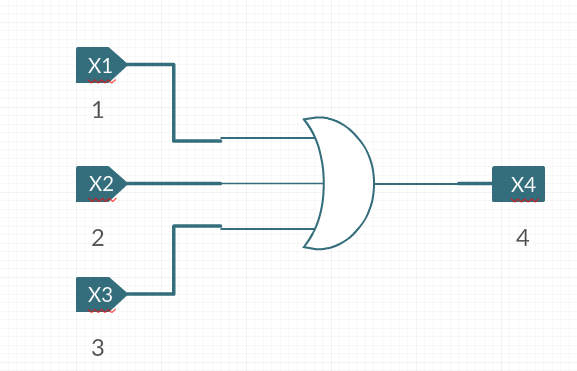
\includegraphics[width=0.5\textwidth]{3-input-or-ul.png}}
	\subfloat[]{\label{fig:or-ur}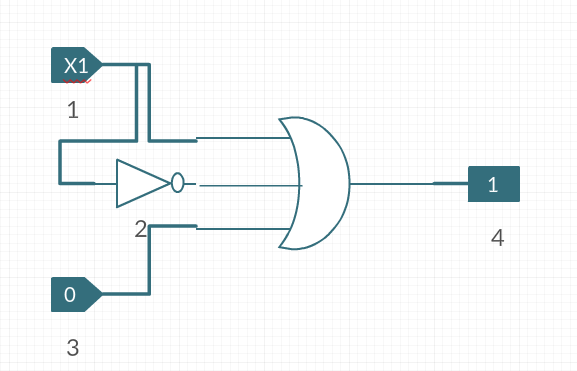
\includegraphics[width=0.5\textwidth]{3-input-or-ur.png}}
	\newline
	\subfloat[]{\label{fig:or-ll}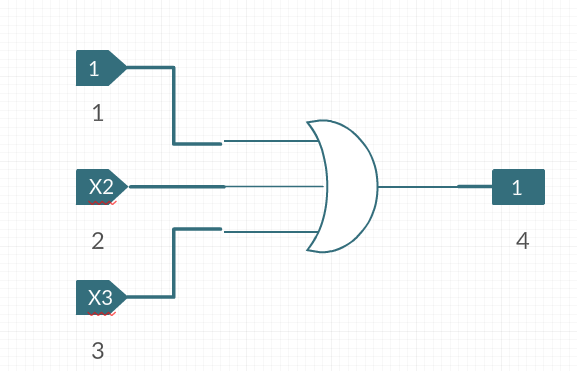
\includegraphics[width=0.5\textwidth]{3-input-or-ll.png}}
	\subfloat[]{\label{fig:or-lr}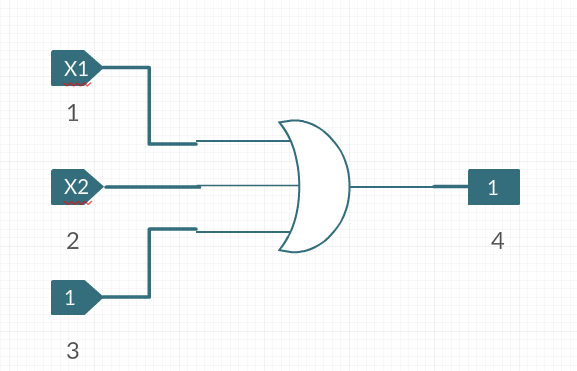
\includegraphics[width=0.5\textwidth]{3-input-or-lr.png}}
	\label{fig:or-group}
	\caption[Multi-input OR Gates]{Various Multi-input OR Gate Configurations}
\end{figure}

\subsection{Controlling Values}

\subsection{Major Changes}

\section{XOR}

\subsection{Order of Inputs}

\begin{figure}[h]	
	\subfloat[]{\label{fig:xor-ul}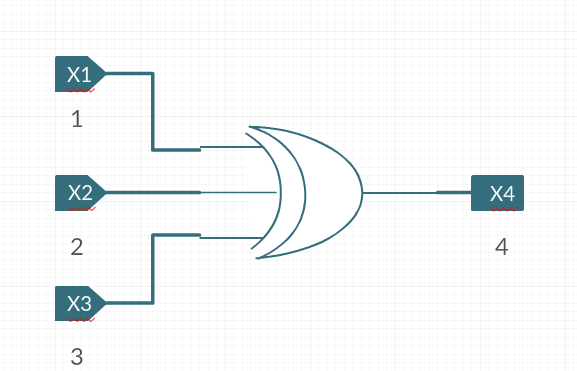
\includegraphics[width=0.5\textwidth]{3-input-xor-ul.png}}
	\subfloat[]{\label{fig:xor-ur}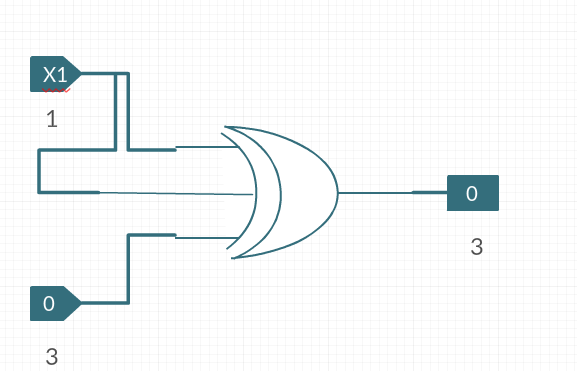
\includegraphics[width=0.5\textwidth]{3-input-xor-ur.png}}
	\newline
	\subfloat[]{\label{fig:xor-ll}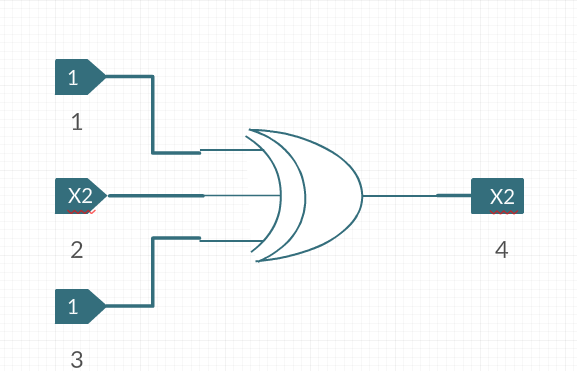
\includegraphics[width=0.5\textwidth]{3-input-xor-ll.png}}
	\subfloat[]{\label{fig:xor-lr}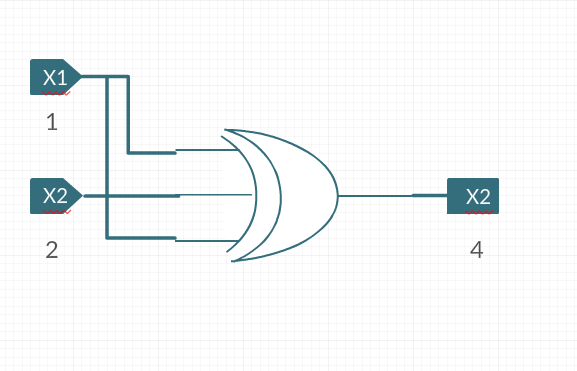
\includegraphics[width=0.5\textwidth]{3-input-xor-lr.png}}
	\label{fig:xor-group}
	\caption[Multi-input XOR Gates]{Various Multi-input XOR Gate Configurations}
\end{figure}

\subsection{Restoring X's}

\chapter{X-Trees}
\label{sec:xtree}

\section{Overview}

\begin{figure}[h]
	\centering
	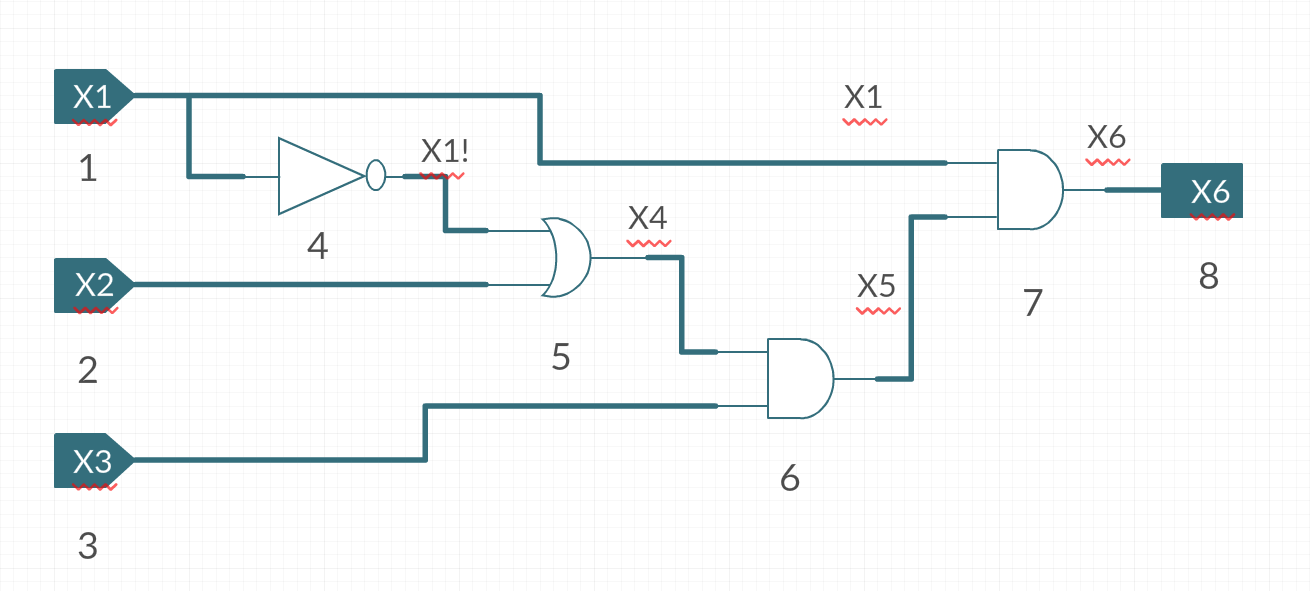
\includegraphics[width=0.7\textwidth]{xtree-circuit.png}
	\caption[X-Tree Circuit]{The circuit used in the example simulation}
	\label{fig:xtree-ckt}
\end{figure}

\begin{figure}[h]
	\centering
	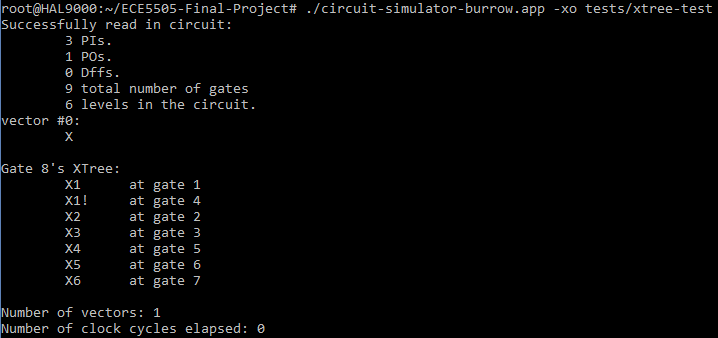
\includegraphics[width=0.7\textwidth]{sim-output.png}
	\caption[X-Tree Output]{An example of the X-Tree output of the simulator}
	\label{fig:sim-output}
\end{figure}

\section{Effects on Gates}

\subsection{AND/OR}

\subsection{XOR}

\chapter{User Interface}
\label{sec:ui}

\section{Overview}

\section{X-Trees}

\begin{figure}[h]
	\centering
	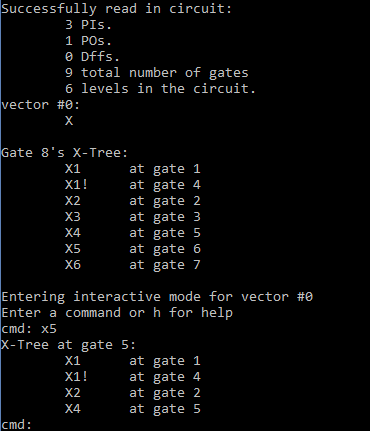
\includegraphics[width=0.7\textwidth]{sim-xtree-cmd.png}
	\caption[UI X-Tree Viewer]{An example of the user interface and how to observe the X-Tree of any gate in the circuit}
	\label{fig:sim-xtree-cmd}
\end{figure}

\section{Controlling Gates}

\begin{figure}[h]
	\centering
	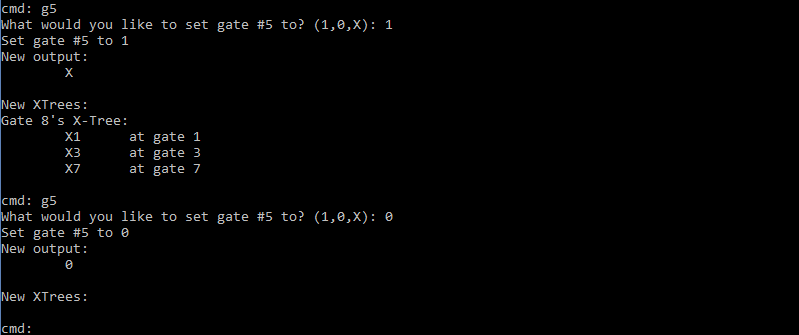
\includegraphics[width=0.7\textwidth]{sim-gate-cmd.png}
	\caption[UI Gate Controller]{An example of the user interface and how to force a value on the output of a gate}
	\label{fig:sim-gate-cmd}
\end{figure}

\pdfbookmark{Bibliography}{bib}
\bibliographystyle{myIEEEtran}
\bibliography{references}

\appendix

% In LaTeX, each appendix is a "chapter"
% \chapter{Program Source}


\end{document}
